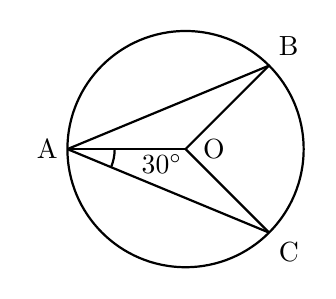
\begin{tikzpicture}[scale=1]

  % Define the center of the circle
  \coordinate (O) at (0,0);

  % Define the radius of the circle
  \def\R{1.5}

  % Draw the circle
  \draw[thick] (O) circle (\R);

  % Define the vertices on the circle
  % A is on the left
  \coordinate (A) at (180:\R);
  % B is top right
  \coordinate (B) at (45:\R);
  % C is bottom right
  \coordinate (C) at (315:\R);

  % Draw the line segments OA, OB, OC
  \draw[thick] (O) -- (A);
  \draw[thick] (O) -- (B);
  \draw[thick] (O) -- (C);

  % Draw the chords AB and AC
  \draw[thick] (A) -- (B);
  \draw[thick] (A) -- (C);

  % Draw the angle arc for 30° at A (between AC and AO)
  % Angle of AO is 0 from A
  % Angle of AC is -22.5 from A (since triangle AOC is isosceles with central angle 135°)
  \draw[thick] (A) ++(-22.5:0.6) arc (-22.5:0:0.6);
  \node at (-0.3, -0.19) {$30^\circ$};

  % Add labels for the points
  \node[left] at (A) {A};
  \node[above right] at (B) {B};
  \node[below right] at (C) {C};
  \node[right] at (0.1, 0) {O};

\end{tikzpicture}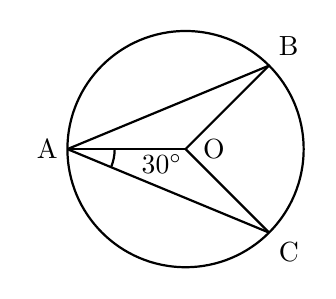
\begin{tikzpicture}[scale=1]

  % Define the center of the circle
  \coordinate (O) at (0,0);

  % Define the radius of the circle
  \def\R{1.5}

  % Draw the circle
  \draw[thick] (O) circle (\R);

  % Define the vertices on the circle
  % A is on the left
  \coordinate (A) at (180:\R);
  % B is top right
  \coordinate (B) at (45:\R);
  % C is bottom right
  \coordinate (C) at (315:\R);

  % Draw the line segments OA, OB, OC
  \draw[thick] (O) -- (A);
  \draw[thick] (O) -- (B);
  \draw[thick] (O) -- (C);

  % Draw the chords AB and AC
  \draw[thick] (A) -- (B);
  \draw[thick] (A) -- (C);

  % Draw the angle arc for 30° at A (between AC and AO)
  % Angle of AO is 0 from A
  % Angle of AC is -22.5 from A (since triangle AOC is isosceles with central angle 135°)
  \draw[thick] (A) ++(-22.5:0.6) arc (-22.5:0:0.6);
  \node at (-0.3, -0.19) {$30^\circ$};

  % Add labels for the points
  \node[left] at (A) {A};
  \node[above right] at (B) {B};
  \node[below right] at (C) {C};
  \node[right] at (0.1, 0) {O};

\end{tikzpicture}